\chapter{Taux de réaction de résonances}
\section{Section efficace de résonance}
	\subsection{Section efficace effective}
	Au premier chapitre (*nostalgie*), nous avions vu que la section efficace était fonction de la
	\textit{vitesse relative} entre le neutron et le noyau cible. Il doit donc y avoir un impact du 
	mouvement thermique sur les noyaux lourds qui ne peuvent plus être considérés comme immobiles 
	(ce que nous avions supposé au second chapitre).\\
	
	La \textit{probabilité par unité de temps d'avoir une interaction entre un neutron et un noyau 
	lourd} est donné par
	\begin{equation}
	N\sigma (|\bar v - \bar V|).|\bar v - \bar V|
	\end{equation}
	où $\bar v$ et $\bar V$ sont les vitesses \textbf{absolues} du neutron et du noyau lourd. Le 
	\textit{taux de réaction} va alors être un peu modifié 
	\begin{equation}
	R = \int\limits_{\bar v}  n(\bar v)d\bar v\int\limits_{\bar V}  N\sigma (|\bar v - \bar V|).|\bar v
	 - \bar V|P(V)d\bar V
	\end{equation}
	La densité neutronique est une fonction de la vitesse absolue des neutrons. S'il y a de 
	l'agitation thermique, c'est qu'il y a une distribution sur les vitesses absolue des noyaux ;
	$P(V)$. Ainsi, le taux de réaction est le produit de la densité avec $\sigma$ que l'on intégrait
	sur toutes les vitesses mais ici il faut en plus intégrer sur la distribution de probabilité des
	vitesses des noyaux cibles. \\
	
	En considérant que $P$ est une fonction densité de probabilité due au mouvement thermique et que
	$\sigma$ est une fonction scalaire de la vitesse, on défini la \textbf{section efficace
	effective}\ \\
	
	\cadre{\begin{equation}
	v{\sigma _{eff}}(v) = \int\limits_{\bar V}   \sigma (|\bar v - \bar V|).|\bar v - \bar V|P(V)d\bar
	 V
	\end{equation}}\ 
	
	Il s'agit d'une sorte d'équivalent : ça fait apparaître quelque chose qui dépend uniquement de la
	vitesse des neutrons et c'est dans cette intégrale que su trouve tout l'impact de la variation 
	de la vitesse des noyaux cibles. Pour retrouver la même écriture (sans approximation) du taux 
	de réaction
	\begin{equation}
	R = \int_o^\infty     N{\sigma _{eff}}(v)\varphi (v)dv
	\end{equation}
	où le flux $\varphi (v) = \int\limits_{4\pi }  vn(\bar v){v^2}d\bar \Omega $  dépend de la vitesse
	scalaire, il faut "corriger" la section efficace et c'est le rôle de la section efficace 
	effective.\\
	
	Considérons quelques cas particulier afin de voir l'impact de l'ajout de cet indice $eff$ à la 
	section efficace. Soit $\bar v_r = \bar v -\bar V$
	\begin{enumerate}
	\item Nous avions vu au chapitre 1 que bien en deçà d'un pic de résonance, le comportement 
	de la section microscopique était en $v^{-1}$ (Breit-Wigner pour $E\ll E_0$). Si $\sigma = 
	c/v_r$ :
	\begin{equation}
	{\sigma _{eff}}(v) = \frac{1}{v}\int\limits_{\bar V}  \frac{c}{{|\bar v - \bar V|}}.|\bar v -
	 \bar V|P(V)d\bar V = \frac{c}{v}
	\end{equation}
	Le profil reste inchangé !
	\item Si $\sigma$ varie lentement et pour des énergies suffisamment élevée que pour être loin 
	des zones de résonances : $v_r \approx v$ (la vitesse des noyaux lourds est négligeable)
	\begin{equation}
	{\sigma _{eff}}(v) = \frac{1}{v}\int\limits_{\bar V}    \sigma (v)vP(V)d\bar V = \sigma (v)
	\end{equation}
	On retrouve le résultat de départ où $\sigma_{eff}=\sigma$.
	\item Si l'énergie d'un neutron est basse par rapport à la zone thermique : $v_r\approx V$ 
	(la vitesse des neutrons est négligeable)
	\begin{equation}
	{\sigma _{eff}}(v) = \frac{1}{v}\int\limits_{\bar V}   \sigma (V)VP(V)d\bar V =
	 \frac{{{c^{ste}}}}{v}
	\end{equation}
	Ce résultat est \textbf{indépendant} de $\sigma$ !  On a totalement perdu la trace du départ
	du $\sigma_{eff}$.
	\end{enumerate}
	
	Analysons ces cas de figure. Le premier cas est bien acceptable, le second est totalement 
	correct mais le troisième nous montre qu'il faut faire attention même si "\textit{dans l'ensemble 
	c'est bien, on a pas fait trop n'importe quoi}".
	
	\subsection{Effet Doppler}
	Commençons par une petite remarque à propos de la fonction $v{\sigma _{eff}}(v)$. Celle-ci est
	obtenue par convolution entre $|\bar v|.\sigma(|\bar v|)$ et $P(V)$ : cette convolution cause
	un élargissement des pics de résonance.
	
	\subsubsection{Profil Doppler}
	Intéressons-nous au profil de Doppler pour une résonance centrée sur $E_0 \gg k_BT$, où 
	$E_0$ est l'énergie du mouvement relatif. Pour modéliser le spectre de l'agitation thermique, 
	nous allons considérer une distribution maxwellienne
	\begin{equation}
	P(V)d\bar V = {\left( {\frac{M}{{2\pi kT}}} \right)^{3/2}}.{e^{ - \frac{{M{V^2}}}{{2kT}}}}d\bar V
	\end{equation}
	La section efficace effective associée à ça c'est globalement $1/v$ que multiplie l'intégrale
	sur les vitesses relatives où l'on remplace $v$ par la vitesse relative (afin d'obtenir une 
	sorte de moyenne)
	\begin{equation}
	{\sigma _{eff}}(v) = {\left( {\frac{M}{{2\pi kT}}} \right)^{3/2}}.\frac{1}{v}\int\limits_{{{\bar
	 v}_r}}   {v_r}\sigma ({v_r}){e^{ - \frac{{M|\bar v - {{\bar v}_r}{|^2}}}{{2kT}}}}d{\bar v_r}
	\end{equation}
	A la grosse louche, nous avons
	\begin{equation}
	\int _{\bar v_r} \dots d\bar v_r
	\end{equation}
	où $d\bar v_r \equiv v_r^2 dv_r d\bar\Omega = v_r^2dv_r2\pi d\mu$. Par changement de variable, 
	l'exponentielle devient $e^{\frac{M}{2kT}(v^2+v_r^2-2\mu v v_r)}$. Comme nous savons que 
	$\mu$ varie de -1 à +1, on peut séparer l'exponentielle en deux : une positive et une négative
	\begin{equation}
	{\sigma _{eff}}(v) = {\left( {\frac{M}{{2\pi kT}}} \right)^{1/2}}.\frac{1}{{{v^2}}}\int_o^\infty  
	 v_r^2\sigma ({v_r})\left( {{e^{ - \frac{{M{{(v - {v_r})}^2}}}{{2kT}}}} - {e^{ - \frac{{M{{(v +
	 {v_r})}^2}}}{{2kT}}}}} \right)d{v_r}
	\end{equation}
	Nous allons négliger la seconde exponentielle par rapport à la première. En effet, nous regardons
	sur un pic de résonance particulier, la somme des vitesses va être négligeable par rapport à la 
	différence des vitesses relatives sur un même pic
	\begin{equation}
	{\sigma _{eff}}(v) \cong {\left( {\frac{M}{{2\pi kT}}} \right)^{1/2}}.\frac{1}{{{v^2}}}\int_o^
	\infty    v_r^2\sigma ({v_r}){e^{ - \frac{{M{{(v - {v_r})}^2}}}{{2kT}}}}d{v_r}
	\end{equation}
	Pour résoudre cette équation, faisons l'approximation suivante
	\begin{equation}
	v - {v_r} \approx \frac{{{v^2} - {v_r}^2}}{{2{v_r}}}
	\end{equation}
	Nous allons introduire quelques paramètres réduits ainsi que le paramètre $\Delta$ qui va 
	reprendre "\textit{un peu tout le brol qui trainant devant}. Celui-ci possède deux 
	caractéristiques : la masse réduite et l'absolue, mais le tout à une dimension d'énergie. Il 
	s'agit d'une largeur de raie (ici Doppler) qui augmente avec la température
	\begin{equation}
	\mu  = \frac{{mM}}{{M + m}},\qquad\qquad \tilde E = \frac{{\mu {v^2}}}{2},\qquad\qquad
	{E_r} = \frac{{\mu {v_r}^2}}{2},\qquad\qquad \Delta  = \sqrt {\frac{{4kT\mu {E_o}}}{M}} 
	\end{equation}
	En substituant
	\begin{equation}
	{\sigma _{eff}}(\tilde E) = \frac{1}{{\sqrt \pi  \Delta }}.\frac{{\sqrt {{E_o}} }}{{\tilde E}}
	\int_o^\infty    \sqrt {{E_r}} \sigma ({E_r}){e^{ - \frac{{{{(\tilde E - {E_r})}^2}}}{{{\Delta
	 ^2}{\textstyle{{{E_r}} \over {{E_o}}}}}}}}d{E_r}
	\end{equation}
	Quelques petites opération arithmétiques plus tard
	\begin{equation}
	{\sigma _{eff}}(\tilde E) \cong \frac{1}{{\sqrt \pi  \Delta }}\int_o^\infty    \sigma ({E_r}){e^{
	 - \frac{{{{(\tilde E - {E_r})}^2}}}{{{\Delta ^2}}}}}d{E_r}
	\end{equation}
	En restant dans le même genre d'approximation, nous montrons ici que la variation de l'énergie
	du mouvement relatif sera surtout marquée au pic.
	
	

	\subsection{Comparaison avec le profil naturel}
	Posons
	\begin{equation}
	x = \frac{{\tilde E - {E_o}}}{{\Gamma /2}},\qquad\qquad 
	y = \frac{{{E_r} - {E_o}}}{{\Gamma /2}},\qquad\qquad \theta  = \frac{\Gamma }{\Delta }
	\end{equation}		
	où $\Gamma$ est la largeur d'un pic. On peut ré-écrire $\sigma_{eff}$ :\\
	
	\cadre{\begin{equation}
	{\sigma _{eff}}(x) \cong \frac{\theta }{{2\sqrt \pi  }}\int_{ - \infty }^\infty   \sigma (y)
	{e^{ - \frac{{{\theta ^2}{{(x - y)}^2}}}{4}}}dy
	\label{eq:CWNP}
	\end{equation}}\ \\
	
	En faisant passer chacun des termes de la première colonne du tableau ci-dessous dans 
	l'expression \eqref{eq:CWNP} et avec l'aide des fonctions de Bethe-Placzek\footnote{Quelques 
	propriétés de ces fonctions sont données au slide 7.} on peut obtenir les différents profil 
	Doppler
	
	\begin{center}
	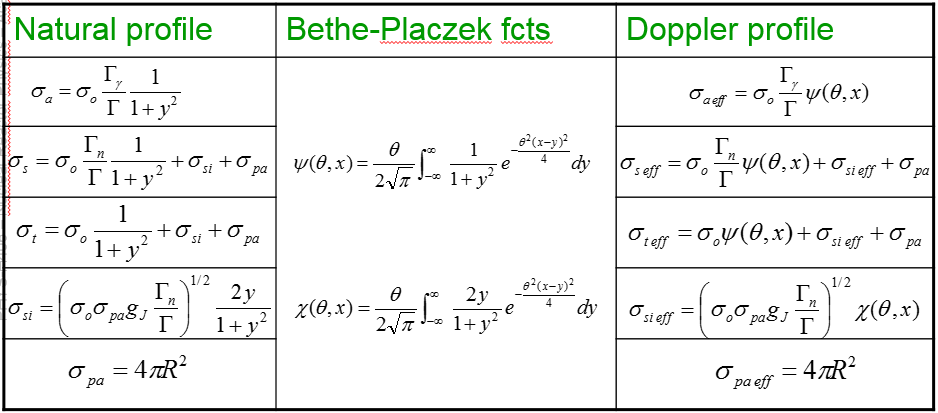
\includegraphics[scale=0.65]{ch8/image1}
	\captionof{table}{ }
	\end{center}
	
\section{Intégrale de résonance}
Ce n'est plus une surprise : le taux d'absorption dans un pic de résonance est donné par
\begin{equation}
{R_a} = \int\limits_{R\'e s}  {\Sigma _a}(u)\varphi (u)du
\end{equation}
On \textit{définit} alors l'\textbf{intégrale de résonance} \\

\cadre{\begin{equation}
I \equiv \int\limits_{R\'e s}    {\sigma _a}(u)\frac{{\varphi (u)}}{{{\varphi _{as}}}}du
\end{equation}
où $\varphi_{as}$ est le flux asymptotique, c'est-à-dire sans résonance.}\ \\

Celle-ci à les unité d'une section efficace qui fait apparaître l'intégrale de cette section 
efficace d'absorption sur cette résonance multipliée par le flux observé au sein même de cette 
résonance sur le flux asymptotique au delà de cette résonance.\\

On peut voir le taux d'absorption $R_a$ comme un flux asymptotique au delà de la résonance, une 
densité isotopique et une \textit{section efficace équivalente} $I$ donné par l'intégrale de 
résonance
\begin{equation}
{R_a} = NI{\varphi _{as}}
\end{equation}
On voit ainsi apparaître une dépression du flux dans la résonance mais la densité de ralentissement
est elle plus ou moins constante sur le $\Delta u$ d'une unique résonance. En bref, l'impact d'une
seule résonance sur la densité de ralentissement ne sera pas énorme et on peut pourl'instant 
négliger cette petite différence. Si l'absorption est faible ou si $\xi = \gamma$ :
\begin{equation}
q(u) = \xi {\Sigma _t}(u)\varphi (u) \approx q
\end{equation}
La probabilité anti-trappe reste aux alentours de 0.87. Avant la résonance nous avons 
$q=\xi\Sigma_p\varphi_{as}$ car $\Sigma_t\approx \Sigma_p = c^{te}$ où $\Sigma_p$ est le 
scattering de potentiel.  On en tire\footnote{Le slide 9 donne des exemples d'applications.}\\

\cadre{
\begin{equation}
I \equiv \int\limits_{R\'e s}    {\sigma _a}(u)\frac{{{\Sigma _p}}}{{{\Sigma _t}(u)}}du,\qquad
\qquad\qquad {R_a} = q\frac{{NI}}{{\xi {\Sigma _p}}}
\end{equation}}
	
	
\section{Intégrale de résonance - réacteur thermique homogène}
	\subsection{Dilution infinie}
	Il s'agit du cas où seulement très peu d'atomes sont absorbés : $\varphi(u) = \varphi_{as}(u)$.
	Dans ce cas, l'intégrale de résonance devient
	\begin{equation}
	{I_\infty } = \int\limits_{R\'e s}  {\sigma _{a\;eff}}(E)\frac{{dE}}{E}
	 \cong \frac{\Gamma }{{2{E_o}}}\int\limits_{R\'e s}  {\sigma _{a\;eff}}(y)dy = \frac{{{\Gamma _
	 \gamma  }}}{{2{E_o}}}{\sigma _o}\pi 
	\end{equation}
	Plus l'énergie est petite, plus l'intégrale sera grande et donc plus on va vers le thermique, plus
	l'impact des résonance est marqué. On va approximer cette intégrale par deux méthodes

	\subsection{Approximations $NR$ et $NRIA$}
	Ces approximations sont utilisées pour calculer ce qui se passe dans le cas de mélanges ($NR$
	signifie "\textit{narrow resonance}"). Considérons un mélange homogène de modérateurs $m$ 
	non-absorbant avec un potentiel de scattering $\Sigma_m$ ainsi que $N$ (densité) noyaux 
	absorbants $a$ :
	\begin{equation}
	\left\{\begin{array}{ll}
	{\Sigma _a} &\DS= N{\sigma _a}\\
	{\Sigma _t} &\DS= N{\sigma _t} + {\Sigma _m}\\
	{\Sigma _p} &\DS= N{\sigma _{pa}} + {\Sigma _m}
	\end{array}\right.
	\end{equation}
	où les section efficaces microscopiques par atome absorbant sont données par
	\begin{equation}
	\left\{\begin{array}{ll}
	{\sigma _m} &\DS= \frac{{{\Sigma _m}}}{N}\\
	{\sigma _{tot}} &\DS= \frac{{{\Sigma _t}}}{N} = {\sigma _t} + {\sigma _m}\\
	{\sigma _p} &\DS= \frac{{{\Sigma _p}}}{N} = {\sigma _{pa}} + {\sigma _m}
	\end{array}\right.
	\end{equation}
	
	\subsubsection{Approximation $NR$}
	Dans cette approximation, on suppose que la résonance est étroite, c'est-à-dire que la 
	largeur de raie associée à cette résonance est petite par rapport au taux de variations des 
	énergies moyennes que l'on va avoir pour les collisions des neutrons avec les noyaux lourds du 
	milieu absorbant
	\begin{equation}
	\Gamma \ll < E' - E{ > _m},\qquad\qquad \Gamma \ll \langle E'-E\rangle_a
	\end{equation}
	C'est-à-dire, en terme de modération que $q_i\gg \Delta u_{res}$ ce qui implique que
	\begin{equation}
	F(u) = \sum\limits_i    \int_{u - {q_i}}^u    \frac{{{e^{u' - u}}}}{{1 - {\alpha _i}}}{\Sigma
	_{si}}(u')\varphi (u')du'  \cong \sum\limits_i  \int_{u - {q_i}}^u  \frac{{{e^{u' - u}}}}{{1 -
	{\alpha _i}}}du'{\Sigma _{pi}}{\varphi _{as}} = {\Sigma _p}{\varphi _{as}}
	\end{equation}
	où $F(u)$ est l'équation de ralentissement en milieu infini (cf. chapitre 7). Par définition, 
	nous avions établi que $F(u) = {\Sigma _t}(u)\varphi (u)$. Il en vient que 
	$\frac{{\varphi (u)}}{{{\varphi _{as}}}} = \frac{{{\sigma _p}}}{{{\sigma _{tot}}(u)}}$. On 
	peut sortir de l'intégrale tout ce qui est au delà du comportement asymptotique pour obtenir 
	l'intégrale de résonance en approximation $NR$ \\
	
	\cadre{
	\begin{equation}
	{I^{NR}} = \int\limits_{R\'e s} \frac{{{\sigma _a}(u){\sigma _p}}}{{{\sigma _{tot}}(u)}}du
	\end{equation}}
	
	\subsubsection{Approximation $NRIA$}
	Ici nous sommes toujours proche des résonances mais en plus les noyaux lourds le sont vraiment
	($A$ tend vers l'infini) : ils ne contribuent pas au ralentissement.
	\begin{equation}
	\Gamma \ll \langle E'-E\rangle_m,\qquad\qquad\qquad \langle E'-E\rangle_a = 0
	\end{equation}
	Pour le terme lié au noyau lourd, il ne faut considérer que le pic de Dirac associé à ce 
	milieu la : $K(u) = \delta(u)$ pour l'absorbant. Comme 
	$F(u) = {\Sigma _t}(u)\varphi (u) = {\Sigma _{sa}}(u)\varphi (u) + {\Sigma _m}{\varphi _{as}}$ 
	on peut en déduire l'intégrale de résonance\\
	
	\cadre{\begin{equation}
	{I^*} = \frac{{\pi {\sigma _o}{\Gamma _\gamma }}}{{2{E_o}}}\sqrt {\frac{{{\beta ^*}}}{{{\beta ^*}
	 + 1}}}
	\end{equation}}\ \\
	
	Si l'on cherche les profils naturels pour les sections efficaces, que ce soit en $NR$ ou $NRIA$, 
	en triturant suffisamment les deux expressions on peut les ramener à une forme unique $I^*$ avec 
	un paramètre $\beta$ introduit variant selon l'approximation
	\begin{equation}
	{I^*} = \frac{{\pi {\sigma _o}{\Gamma _\gamma }}}{{2{E_o}}}\sqrt {\frac{{{\beta ^*}}}{{{\beta ^*}
	 + 1}}} 
	\end{equation}
	avec ${\beta ^{NR}} = \frac{{{\sigma _{pa}} + {\sigma _m}}}{{{\sigma _o}}}$ et 
	${\beta ^{NRIA}} = \frac{{{\sigma _m}}}{{{\sigma _o}}}\frac{\Gamma }{{{\Gamma _\gamma }}}$.\\
	
	\textsc{Remarque}.\\
	Le profil de Doppler est obtenu via
	\begin{equation}
	{I^*} = \frac{{{\sigma _o}{\Gamma _\gamma }}}{{{E_o}}}{\beta ^*}J(\theta ,{\beta ^*})
	\end{equation}
	où 
	\begin{equation}
	J(\theta ,\beta ) = \frac{1}{2}\int_{ - \infty }^\infty  \frac{{\psi (\theta ,x)}}{{\beta  +
	 \psi (\theta ,x)}}dx  = \int_o^\infty     \frac{{\psi (\theta ,x)}}{{\beta  + \psi (\theta ,x)}}
	 dx
	\end{equation}\ 
	
	\begin{wrapfigure}[13]{l}{5cm}
	\vspace{-5mm}
	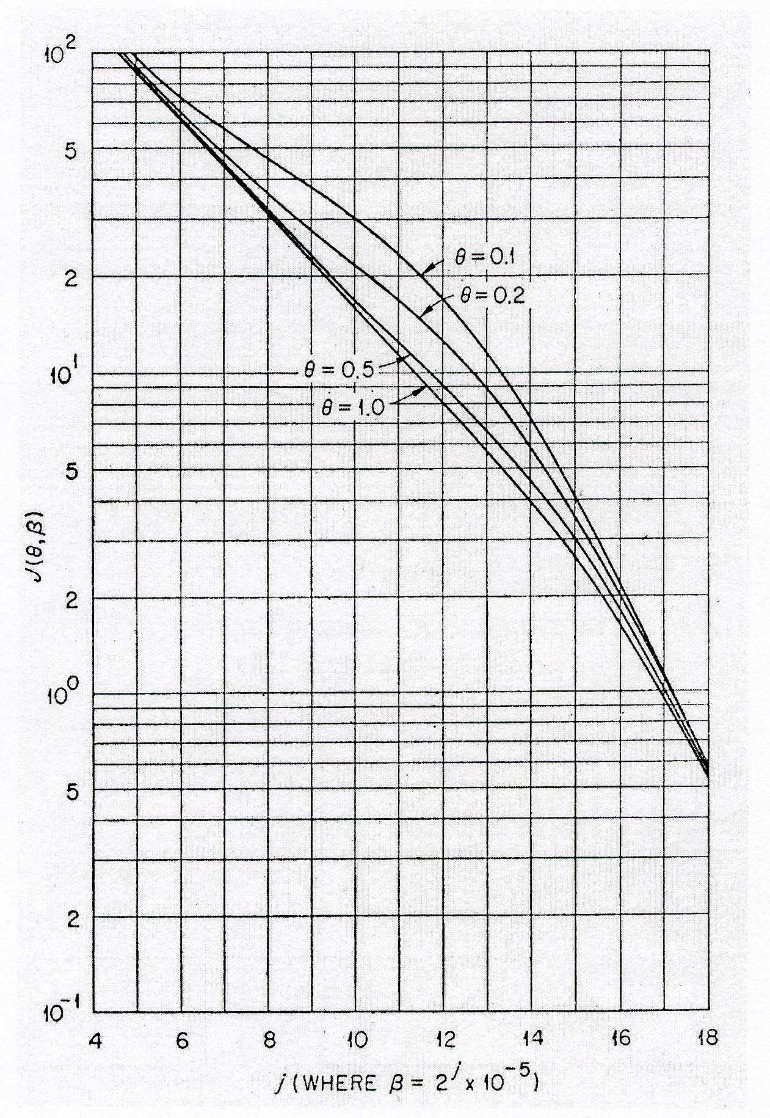
\includegraphics[scale=0.22]{ch8/image2}
	\captionof{figure}{ }
	\end{wrapfigure}
	\textit{Une image vaut mieux qu'un long discours}. Ci-contre, la représentation de $J$ en fonction
	de $\beta$ pour une série de valeurs différentes de $\theta$. Nous savons que $\Delta$, la 
	largeur de Doppler, augmente avec la température en $\sqrt{T}$ : si $\theta$ diminue (augmentation
	de la température), $J$ augmente.\\
	
	La dernière expression nous montre bien que si $\theta$ diminue ($T$ augmente) $J$ augmente. 
	Forcément si la température augmente, l'intégrale de résonance va augmenter, la probabilité 
	anti-trappe va diminuer, $k_{eff}$ va diminuer et donc le flux et la température également. C'est
	comme ceci que l'on peut réguler le modérateur : une rétroaction sur $T$.
	
	\newpage
	\subsubsection{Choix de l'approximation ?}
	Pour des cas pratique ou la largeur de résonance $\Gamma_p$ est telle que $\sigma_{B-W}>
	\sigma{pa}$, le choix se fait en comparant la modération moyenne due à l'absorbant
	\begin{equation}
	\left\{\begin{array}{lll}
	\Gamma_p &< (1-\alpha_a)E_0&\qquad\Rightarrow NR\\
	\Gamma_p &> (1-\alpha_a)E_0&\qquad\Rightarrow NRIA
	\end{array}\right. 
	\end{equation}
	
	Pour les cas intermédiaire, on peut écrire 
	\begin{equation}
	\left\{\begin{array}{ll}
	\beta  &\DS= \frac{{{\sigma _m} + \lambda {\sigma _{pa}}}}{{{\sigma _o}}}\frac{\Gamma }{{{\Gamma _
	\gamma } + \lambda {\Gamma _n}}}\vspace{2mm}\\
	\dfrac{{\varphi (u)}}{{{\varphi _{as}}}} &\DS= \frac{{{\sigma _m} + \lambda {\sigma _{pa}}}}
	{{{\sigma	 _a} + {\sigma _m} + \lambda {\sigma _{pa}}}}\
	\end{array}\right.
	\end{equation}
	où $\lambda=0$ en $NRIA$ et $\lambda=1$ en $NR$. La méthode de Goldstein-Cohen donne des 
	valeurs intermédiaire de $\lambda$ pour l'équation de ralentissement :
	\begin{equation}
	{\Sigma _t}(u)\frac{{\varphi (u)}}{{{\varphi _{as}}}} = \int_{u - {q_o}}^u    \frac{{{e^{u' -
	 u}}}}{{1 - {\alpha _o}}}{\Sigma _{so}}(u')\frac{{\varphi (u')}}{{{\varphi _{as}}}}du' + {\Sigma
	  _m}
	\end{equation}
	
\section{Intégrale de résonance - réacteur thermique hétérogène}
	\subsection{Auto-protection géométrique}
	\begin{wrapfigure}[5]{r}{2cm}
	\vspace{-8mm}
	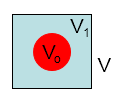
\includegraphics[scale=0.7]{ch8/image3}
	\captionof{figure}{ }
	\end{wrapfigure}	
	Notons que le dessin ci-contre représente une coupe d'un crayon de combustible avec le chenal
	qu'il y a autour.

	\subsubsection{En dehors des résonances}
	Le flux est spatialement uniforme
	\begin{equation}
	{\varphi _{as}} = \dfrac{q}{{\overline {\xi {\Sigma _p}} }}
	\end{equation}
	où $\DS\overline {\xi {\Sigma _p}}  = \frac{{{\xi _o}{\Sigma _{po}}{V_o} + {\xi _1}{\Sigma _{p1}}
	{V_1}}}{V}$. \\
	\textsc{Remarque}. Pour un combustible partiellement modéré : ${\xi _o}{\Sigma _{po}} = {\xi _a}
	{\Sigma _{pa}} + {\xi _m}{\Sigma _m}$
	
	\subsubsection{En dehors des résonances}
	Les neutrons ont des distances un peu plus importantes que les deux volumes et passent d'un des
	milieux à l'autre. On va ainsi avoir une forte dépression du flux dans $V_0$ causant une forte
	diminution de l'intégrale de résonance\footnote{Pourquoi ?}. Ceci justifie l'utilisation de 
	réacteurs hétérogènes. En effet, dans le domaine des résonances on aura plus de capture et en 
	plus une auto-protection énergétique exposée précédemment (avec la rétroaction sur $T$.
	
	
	\subsection{Approximations $NR$ et $NRIA$}
	Nous allons faire l'\textit{hypothèse} que les flux $\varphi_k$ sont spatialement constant 
	dans une zone $k$. Pour la résonance, on considère $\varphi_0\neq\varphi_1$. Introduisons 
	$P_k$ comme étant la probabilité qu'un neutrons apparaissant uniformément et de façon 
	isotrope à léthargie $u$ dans la zone $k$ se fasse absorber ou modérer dans une autre zone. \\
	
	Si on considère que l'espace est une répétition systématique de mêmes cellules ($V_0, V_1$), le
	taux de réaction total que l'on aura dans la zone zéro est la partie de l'équation de 
	ralentissement que l'on va observer pondérée par leurs volumes respectifs. Ainsi, on va 
	observer des particules de l'équation de ralentissement dans chacun des milieux ce qui nous 
	donne le ralentissement dans le combustible\\
	
	\cadre{
	\begin{equation}
	{V_o}{\Sigma _{to}}(u){\varphi _o}(u) = (1 - {P_o}){V_o}\int_{u - {q_o}}^u   {K_o}(u - u'){\Sigma
	 _{so}}(u'){\varphi _o}(u')du' + P_1{V_1}\int_{u - {q_1}}^u   {K_1}(u - u'){\Sigma _{s1}}(u')
	 {\varphi _1}(u')du'
	\end{equation}}
	
	\subsubsection{Approximation $NR$}
	L'approximation est la même que précédemment ($q_0, q_1\gg \Gamma$). On va faire sortir la valeur 
	asymptotique car il s'agit seulement d'une singularité à la résonance et écrire l'expression
	suivante\\
	
	\cadre{\begin{equation}
	{V_o}{\Sigma _{to}}(u){\varphi _o}(u) =(1 - {P_o}){V_o}\int_{u - {q_o}}^u  {K_o}(u - u')du'{\Sigma
	 _{po}}{\varphi _{as}}+ {P_1}{V_1}\int_{u - {q_1}}^u    {K_1}(u - u')du'{\Sigma _{p1}}{\varphi
	  _{as}}
	\end{equation}
	où $P_k$ est bien une probabilité de fuite sans collisions.}\ \\
	
	Au chapitre 2, nous avions vu une relation entre $P_0$ et $P_1$ : $\Sigma_{p1}V_1P_1 = 
	\Sigma_{t0}(u)V_0P_0$ que nous avions généraliser pour un ensemble de zones homogènes $V_i$.
	Donc\footnote{?}
	\begin{equation}
	\frac{{{\varphi _o}(u)}}{{{\varphi _{as}}}} = (1 - {P_o})\frac{{{\Sigma _{po}}}}{{{\Sigma _{to}}
	(u)}} + {P_o} = \frac{{{\Sigma _{po}}}}{{{\Sigma _{to}}(u)}} + {P_o}\frac{{{\Sigma _{to}}(u) -
	 {\Sigma _{po}}}}{{{\Sigma _{to}}(u)}}
	\end{equation}
	Considérons l'approximation de Wigner pour $P_0$
	\begin{equation}
	{P_o} = \frac{1}{{1 + {\Sigma _{to}}\bar \ell }}
	\end{equation}
	où $\bar \ell$ est la longueur de corde moyenne dans le carburant (voir annexes). On peut 
	ré-écrire le flux dans la résonance sur le flux asymptotique
	\begin{equation}
	\frac{{{\varphi _o}(u)}}{{{\varphi _{as}}}} = \frac{{{\Sigma _{po}}\bar \ell  + 1}}{{1 + {\Sigma
	 _{to}}\bar \ell }} \equiv \frac{{\Sigma _p^*}}{{\Sigma _t^*}}\quad\text{ où }\quad\left\{
	 \begin{array}{ll}
	\sigma _m^* &\DS= \frac{{\Sigma _m^*}}{N} = \frac{{{\Sigma _m} + 1/\bar \ell }}{N}\vspace{2mm}\\
	\sigma _t^* &\DS= \frac{{\Sigma _t^*}}{N} = {\sigma _t} + \sigma _m^*\vspace{2mm}\\
	\sigma _p^* &\DS= \frac{{\Sigma _p^*}}{N} = {\sigma _{pa}} + \sigma _m^*
	 \end{array}\right.
	\end{equation}
	ou les \textit{section efficaces star} sont lié au modérateur. Après ré-écriture, on retrouve 
	la même expression que précédemment si ce n'est que les sections sont augmentée dans ce cas
	hétérogène par $1/\bar\ell$\\
	
	\cadre{\begin{equation}
	{I^{NR}} = \int\limits_{R\'e s}   \frac{{{\sigma _a}(u)\sigma _p^*}}{{{\sigma _t}(u) + \sigma
	 _m^*}}du
	\end{equation}}
	
	\subsubsection{Approximation $NRIA$}
	C'est cadeau \\
	
	\cadre{\begin{equation}
	{V_o}({\Sigma _a}(u) + {\Sigma _m})\varphi (u) = (1 - {P_o}){V_o}\int_{u - {q_m}}^u   
	{K_m}(u - u')du'{\Sigma _m}{\varphi _{as}} + {P_1}{V_1}{\Sigma _{p1}}{\varphi _{as}}
	\end{equation}
	car l'absorbant ne modère pas.}\ \\
	
	Problème d'approximation, on utilise Wigner et on obtient\\
	
	\cadre{
	\begin{equation}
	{I^{NRIA}} = \int\limits_{R\'e s}    \frac{{{\sigma _a}(u)\sigma _m^*}}{{{\sigma _t}(u) + \sigma
	 _m^*}}du
	\end{equation}}\ \\
	
	Cette forme est similaire à celle du cas homogène. \textit{Bref, on peut retrouver des 
	expressions formellement équivalentes avec des section différentielles de scattering modifiées 
	par rapport à ce que nous avions}. Les théorèmes d'équivalences sont ainsi toujours vérifiées.\\
	
	La fin du chapitre n'est pas à connaître. Je n'ai pas le temps de m'occuper du dernier chapitre, 
	la synthèse se termine donc ici.
	
	\vspace{4cm}
	\begin{center}
	
\includegraphics[scale=0.2]{ch8/fin}
	\end{center}